\documentclass{beamer}

\usepackage[english]{babel}
\usepackage[T1]{fontenc}
\usepackage[utf8]{inputenc}

\usepackage{amsmath}	% math fonts
\usepackage{amsthm}
\usepackage{amsfonts}
\usepackage{amssymb}
\usepackage{marvosym}
\usepackage{mathtools}
\usepackage[SCI,RGB]{aaltologo}
\usepackage{natbib}
\usepackage{booktabs}
\usepackage{multicol}
\usepackage{pifont}

\bibliography{biblib.bib}

\usepackage[figurename=Fig.]{caption}

\usetheme{Sharelatex}
\usepackage[orientation=landscape,size=a0,scale=1.2]{beamerposter}
\setbeamertemplate{caption}[numbered]

%% Author and title information
\title{%
    Probabilistic framework for integration of mass spectrum and retention time information in small molecule identification
}
    
\author[\Letter: eric.bach@aalto.fi]{ % address for correspondence 
    Eric Bach\,$^{\text{1,\Letter}}$, %
    Simon Rogers\,$^{\text{2}}$,    %
    John Williamson\,$^{\text{2}}$,  %
    and Juho Rousu\,$^{\text{1}}$
}
    
\institute[]{%
    $^{\text{1}}$Helsinki institute for Information Technology (HIIT), Department of Computer Science, Aalto University, Espoo, Finland\\
    $^{\text{2}}$School of Computing Science, University of Glasgow, Glasgow, UK
}
    
\date{\today}
%%%%%%%%%%%%%%%%%%%%%%%%%%%%%%

%% Notation
\newcommand{\ms}{MS}
\newcommand{\lc}{LC}
\newcommand{\msone}{\ms$^1$}
\newcommand{\msms}{\ms$^2$}
\newcommand{\lcms}{\lc-\ms}
\newcommand{\lcmsms}{\lc-\msms}

\newcommand{\spec}{x}
\newcommand{\rt}{t}
\newcommand{\cands}{\mathcal{C}}
\newcommand{\seqlength}{N}

%% Commands
\newcommand{\todocite}{\textcolor{red}{\textbf{[CITATION]}}}
\newcommand{\cmark}{\textcolor{aaltoGreen}{\ding{51}}}
\newcommand{\xmark}{\textcolor{aaltoRed}{\ding{55}}}
\newcommand{\pmark}{\textcolor{aaltoOrange}{\ding{108}}}

%%%%%%%%%%%%%%%%%%%%%%%%%%%%%%



\mathtoolsset{showonlyrefs=true}


\begin{document}
\begin{frame}{}

\vfill
  
\begin{columns}[T]

\column{.33\linewidth}
    \begin{block}{{\normalsize Small Molecule Identification in Untargeted Metabolomics}}
    \begin{itemize}
        \item Liquid chromatography (LC) coupled with tandem mass spectrometry (\msms) widely utilized in untargeted metabolomics studies
        \item Challenge: Annotation of \lcms{} peaks with potential molecular structures
        \item Most automated machine learning based approaches utilize \ms{} information only \todocite
        \item \lc{} retention time (RT) is valueable additional information for the annotation \todocite, e.g.
    \end{itemize}
    \end{block}

    \begin{block}{{\normalsize Retention Time (RT) Utilization}}
    \begin{itemize}
     \item Multiple approaches to utilize RT for molecule annotation exist
     \item (utilization of RT information, scalable, cross laboratories (\lc-systems), RT reference free)
     \item[1)] Compare measured RTs with in-house reference RTs \hfill \cmark, \xmark, \xmark, \xmark
     \item[2)] Compare measured RTs with projected reference RTs \hfill \cmark, \xmark, \pmark, \xmark
     \item[3)] Compare measured RTs with predicted RTs \hfill \cmark, \cmark, \pmark, \pmark
     \item[4)] Compare measured RTs with predicted RTs proxies, e.g. LogP \hfill \cmark, \cmark, \cmark, \xmark
%      \item[5)] \framebox{Compare measured retention orders with predicted ones \hfill \pmark, \cmark, \cmark, \cmark}
     \item[5)] Compare measured retention orders with predicted ones \hfill \pmark, \cmark, \cmark, \cmark
     \item Fully supported: \cmark, Partially supported: \pmark, Not supported: \xmark
     \item RT comparison to prune candidate lists or (re)ranking \todocite
    \end{itemize}
    \end{block}

    \begin{block}{{\normalsize \lcms{} Experiment Data and its Formal Representation}}
    \begin{itemize}
        \item Assume data arises from \lcms{} experiment (after peak-picking and alignment)
        \item Available information: \msone{}, RT and (etwaige only for some peaks) \msms
        \item Molecular candidate lists are assumed to be given as well
        \item \msms scores, e.g. MetFrag \todocite or CSI:FingerID \todocite, computed
        \item Data from \lcms{} considered as set of $\seqlength$ \ms{} features:
            \begin{equation}
                \mathcal{D}=\{(\spec_i,\rt_i,\cands_i)\}_{i=1}^\seqlength
            \end{equation}
        \item $\spec_i$: \msms{} spectrum (or \msone{}, if no fragmentation available)
        \item $\rt_i$: Measured RT
        \item $\cands_i$: Potentail molecular annotations for feature $i$, e.g. exact mass search
    \end{itemize}
    \end{block}

% ... end of first column

\column{.33\linewidth}
    \begin{block}{{\normalsize 4. Overall Workflow}}
    \begin{figure}
        \centering
        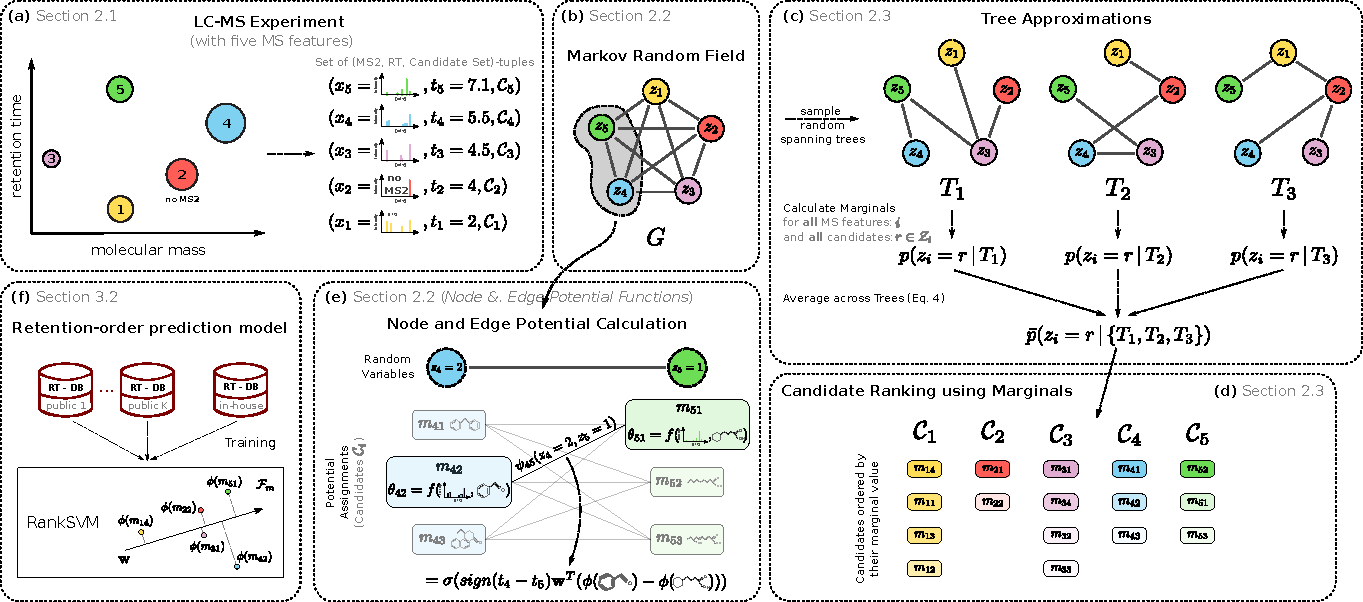
\includegraphics[width=\textwidth]{images/workflow.pdf}
    \end{figure}
    \end{block}

    \begin{block}{{\normalsize Probabilistic Framework to integrate \ms{} and Retention Orders}}
    \begin{itemize}
        \item Definition of a probabilsitic graphical model superimposed on the \lcms{} data
        \item Let $G=(E,V)$ be a complete graph
        \item Nodes $i\in V$ represent the \ms{} features, Edes $(i,j)\in E$ the feature pairs
        \item Association of each node with discrete random variable $z_i\in\mathcal{Z}_i=\{1,\ldots,n_i\}$ ($n_i=|\cands_i|$ number of candidates)
        \item Molecule annotation for complete data $\mathbf{z}=\{z_i\,|\,i\in V\}\in\mathcal{Z}_1\times\ldots\times\mathcal{Z}_\seqlength=\mathbf{Z}$
        \item Intuitively: Random variable denotes which candidate is assigned to each feature.
        \item Pairwise Markov Random Field as probabilsitic model \cite{MacKay2005}:
            \begin{equation}
                p(\mathbf{z})=\frac{1}{Z}\prod_{i\in V}\psi_i(z_i)\prod_{(i,j)\in E}\psi_{ij}(z_i,z_j)
            \end{equation}
        \item Ranking molecular candidates via max-marginals:
            \begin{equation}
                p_{\max}(z_i=r)=\underset{\{\mathbf{z}'\in\mathbf{Z}\,|\,z'_i=r\}}{\max}p(z_i)
            \end{equation}
        \item Intuitively, maxmimum probabilsity a candidate assignment with $z_i=r$ can achive
        \item Rank all candidates $r\in\{1,\ldots,n_i\}$ according to there max-marginals
    \end{itemize}
    \end{block}

    \begin{block}{Node and Edge Potentials}
    \begin{itemize}
        \item Node potential function $\psi_i:\mathcal{Z}_i\rightarrow\mathbb{R}_{>0}$: goodness of the match between measured spectrum $x_i$ and candidates of feature $i$
        \item Edge potential function $\psi_{ij}:\mathcal{Z}_i\times\mathcal{Z}_j\rightarrow\mathbb{R}_{>0}$: consistency between the observed retention order of feature $i$ and $j$ with the predicted retention order of the candidates $z_i$ and $z_j$
    \end{itemize}
    \end{block}



\column{.33\linewidth}

    \begin{block}{{\normalsize Spanning Tree Approximation}}
    \begin{itemize}
        \item Marginal inference intractable in practice due to exponentail sized candidate assignment space $\mathcal{Z}$
        \item Exact inference is feasible if $G$ is tree-like \todocite
        \item Resort to infer the max-marginals a set of trees $\mathbf{T}=\{T_t\}_{t=1}^L$ sampled from $G$
        \item Each tree $T_t=(V,E_t)$ is connected graph with all nodes of $G$ but reduces edges set $E_t\subseteq E$
        \item Avergaged marginals used for ranking
            \begin{equation}
                \bar{p}_{\max}(z_i=r\,|\,\mathbf{T})=\frac{1}{L}\sum_{t=1}^L p_{\max}(z_i=r\,|\,T_t)
            \end{equation}
    \end{itemize}
    \begin{figure}
        \centering
        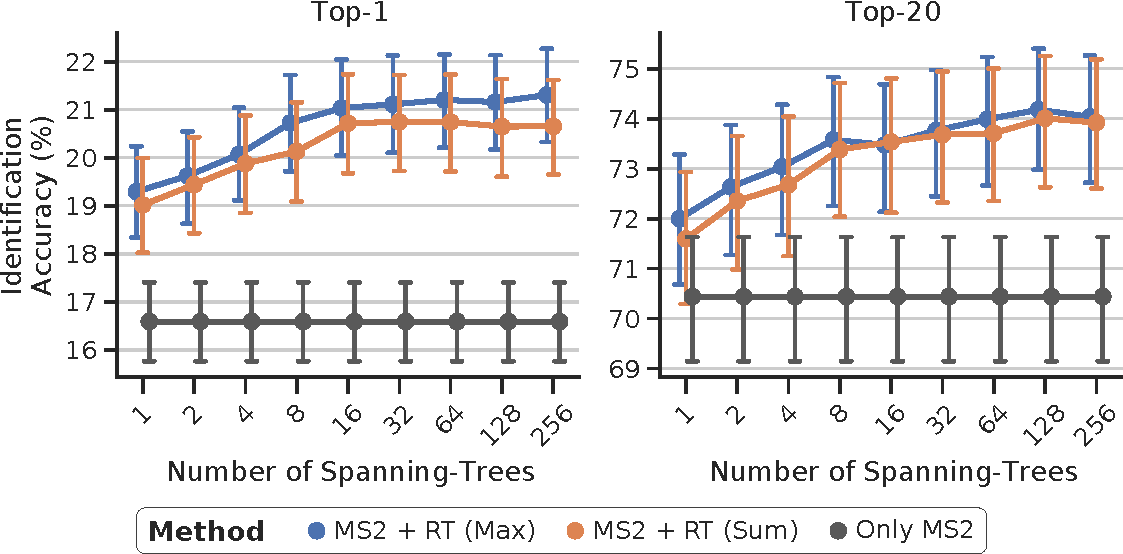
\includegraphics[width=\textwidth]{images/number_of_random_spanning_trees.pdf}
    \end{figure}
    \end{block}


    \begin{block}{{\normalsize 5. Experiments and Results}}
    \end{block}



\vfill

\begin{block}{\small References}
\end{block}
%% <== end of second column

\end{columns}

\vfill

\end{frame}
\end{document}
